\begin{savequote}[8cm]
\textlatin{Neque porro quisquam est qui dolorem ipsum quia dolor sit amet, consectetur, adipisci velit...}

There is no one who loves pain itself, who seeks after it and wants to have it, simply because it is pain...
  \qauthor{--- Cicero's \textit{de Finibus Bonorum et Malorum}}
\end{savequote}

\chapter{\label{ch:1-intro}Introduction} 

\minitoc

In the real world, making informed decisions is crucial. We constantly strive to take actions that lead to desirable outcomes, whether it's a doctor prescribing the most effective treatment for a patient or a company launching a marketing campaign that resonates with its target audience. However, achieving this goal becomes increasingly challenging in the face of uncertainty. Real-world data is often noisy and incomplete, and the systems we interact with are complex and constantly evolving. As machine learning models become more integrated into critical applications, the need for robust decision-making under these challenging conditions becomes paramount.


This thesis explores the key challenges of robust decision-making in machine learning, specifically focusing on the concept of \emph{off-policy evaluation}. Imagine a doctor who wants to assess a new treatment for a disease. Ideally, they would conduct a randomized controlled trial where patients are randomly assigned the new treatment or a standard one. However, such trials can be expensive, time-consuming or worse, ethically problematic. Off-policy evaluation offers a compelling alternative. It allows us to evaluate the performance of a new decision-making policy (the new treatment) using data collected under a different policy (the standard treatment). This eliminates the need for costly experimentation and allows for quicker implementation of potentially more effective strategies.

However, off-policy evaluation presents its own set of challenges. These challenges stem from two main sources of uncertainty:

\begin{itemize}
    \item \textbf{Statistical uncertainty:} This arises from the inherent randomness in the data we have access to and the limitations of the models we use to represent the real world. For instance, the doctor might have a limited number of patients in their historical dataset, and their model might not perfectly capture all the factors that influence a patient's response to treatment.
    \item \textbf{Causal unidentifiability:} In many cases, even with infinite data, it may be impossible to definitively establish the causal effects of actions. This arises due to factors like confounding variables, which can influence both the treatment and the outcome. Imagine the existence of some unmeasured factors, such as a patient's pre-existing conditions, that can influence both their initial treatment and their response to the new treatment. This makes it challenging to isolate the true effect of the new treatment from the influence of these confounding variables.
\end{itemize}
This thesis tackles these challenges head-on, proposing novel methods for off-policy evaluation that address both statistical and causal uncertainties.
Before we go into the specifics of these challenges, we introduce the framework of Contextual Bandits which forms the basis of the setting considered in Chapters \ref{ch:3-mr} and \ref{ch:4-copp}. 

% In the following section, we specifically consider the setting of contextual bandits which provides a powerful framework for 
% will delve deeper into the specifics of these challenges, explore the limitations of existing approaches, and showcase the contributions made by the included research papers.

\section{Contextual Bandits}
Contextual bandits provide a powerful framework for tackling decision-making problems where the effectiveness of an action depends on the specific context in which it is chosen. Imagine a doctor deciding on the best treatment for a patient. The optimal treatment might depend on various factors like the patient's age, medical history, and current symptoms. Contextual bandits allow us to model these complex decision-making scenarios by incorporating the notion of context.

In this setting, we use covariates $X \in \mathcal{X}$ to denote features which encapsulate the contextual information such as the patient's age and medical history, we use $A \in \mathcal{A}$ to represent the action chosen by some real-world agent (such as a doctor), and $Y \in \mathcal{Y}$ to denote the outcome/reward observed as a result of taking action $A$, for example, $Y \in \{0, 1\}$ might represent whether a patient survives ($Y=1$) or not ($Y=0$). The goal of a learner in contextual bandits is to choose actions $A$ for a context $X$ which maximises the reward $Y$. 
% \todo{include causal formulation and connect it with this}

% \begin{importantresultwithtitle}[title=Causal formulation]\noindent
\paragraph{Causal formulation}
 To make the causal dependence of the action on the outcome explicit, we can reformulate the contextual bandits setting using the \emph{potential outcomes framework}. Here, for a given action $a \in \mathcal{A}$ we denote the random variable $Y(a)$ (also known as the potential outcome), as the outcome that \emph{would} occur if the action $a$ is chosen. As random variables, $Y(a)$ may also depend on the initial covariates $X$ and additional randomness which is not explicitly modelled. Moreover, this notation can be reconciled with the conventional contextual bandits setting above by noting that, in the real world where an agent chooses action $A \in \mathcal{A}$ for context $X$, the outcome $Y$ observed is explicitly expressed as $Y(A)$, i.e. $Y=Y(A)$ in the real world. This corresponds to the standard consistency assumption in causal inference and intuitively means that the potential outcome $Y(a)$ is observed in the data when the agent actually chose $A=a$. 
% \end{importantresultwithtitle}

Contextual bandits encapsulate the single-decision regimes where, for each observed context, we make a single action and observe the resulting outcome. This is analogous to a doctor choosing a single treatment for a patient based on their current state. However, many real-world decision-making scenarios involve multiple interventions over time, where each action not only affects the immediate outcome but also influences the context for future decisions. To capture this complexity, we introduce the concept of Dynamic Treatment Regimes (DTRs) in the following section. DTRs extend the framework of contextual bandits to handle sequential decision-making problems, allowing us to model more complex scenarios where interventions unfold over time and the context evolves dynamically.

\section{Dynamic Treatment Regimes}
We consider a setting with a fixed number of decisions per episode (i.e., a fixed time horizon) $T \in \{1, 2, \ldots\}$. For each $t\in \{0, \ldots, T\}$, we assume that the process gives rise to an observation at time $t$, denoted by $X_t$ which takes values in some space $\mathcal{X}_t \coloneqq \R^{\Xspacedim_\tx}$. 
% Moreover, the process can be influenced by some action at time $t \in \{1, \ldots, T\}$ which takes values in some space $\mathcal{A}_t$. 
Moreover, at time $t\in  \{1, \ldots, T\}$ a real-world agent (such as a doctor) chooses an action $A_t$ which takes values in some space $\mathcal{A}_t$. The agent's choice of $A_t$ may depend on the historical observations $(X_0, \ldots, X_{t-1})$ or any additional information not captured in historical observations that the agent can access. For example, in a medical context, the observations may consist of a patient's vital signs, and the actions may consist of possible treatments or interventions that the doctor chooses based on patient history.
% In the real world, the action at time $t$ may be chosen by an agent (such as a doctor) based on the . 
The actions taken up till time $t$, i.e. $(A_1, A_2, \ldots, A_t)$ can influence the future observations $(X_t, X_{t+1}, \ldots, X_T)$. 
This setting describes Dynamic Treatment Regimes, of which the contextual bandits are a special case when $T=1$. 
% To make this concrete, in a robotics context, the observations may consist of all the readings of all the sensors of the robot, and the actions may consist of commands that can be input by an external user. In a medical context, the observations may consist of the vital signs of a patient, and the actions may consist of possible treatments or interventions. 

% \begin{importantresultwithtitle}[title=Causal formulation]\noindent
\paragraph{Causal formulation}
As before, we make the causal dependence of past actions on future observations explicit by modelling the dynamics of the real-world process via the longitudinal potential outcomes framework proposed by Robins. To streamline notation, we will index the spaces using vector notation, so that e.g.\ $\Aspace_{1:t}$ denotes the Cartesian product $\Aspace_1 \times \cdots \times \Aspace_t$, and $a_{1:t} \in \Aspace_{1:t}$ is a choice of $a_1 \in \Aspace_1, \ldots, a_t \in \Aspace_t$.

In this formulation, for each action sequence $a_{1:T} \in \Aspace_{1:T}$, we posit the existence of random variables or \emph{potential outcomes} $X_0, X_1(a_1), \ldots, X_T(a_{1:T})$, where $X_t(a_{1:t})$ takes values in $\Xspace_t$.
We will denote this sequence more concisely as $X_{0:T}(a_{1:T})$.
% Each $\X_\tx(\ax_{1:\tx})$ is referred to as a \emph{potential outcome}.
Intuitively, $X_0$ represents data available before the first action, while $X_{1:T}(a_{1:T})$ represents the sequence of real-world outcomes that \emph{would} occur if actions $a_{1:T}$ were taken successively.
These potential outcomes $X_{1:T}(a_{1:T})$ are also referred to as \emph{interventional outcomes} under the intervention $a_{1:T}$.

As random variables, each $X_{t}(a_{1:t})$ may depend on additional randomness that is not explicitly modelled, and so, in particular, may be influenced by all the previous potential outcomes $X_{0:t-1}(a_{1:t-1})$, and possibly other random quantities.
This models a process whose initial state is determined by external factors, such as when a patient from some population first presents at a hospital, and where the process then evolves according both to specific actions chosen from $\Aspace_{1:T}$ as well as additional external factors.

Just like in the contextual bandits setting, this causal notation can be reconciled with the conventional (non-causal) notation above by noting that, in the real world where an agent chooses action $A_{1:t} \in \mathcal{A}_{1:t}$, the observation at time $t$, $X_{t}$, is explicitly expressed as $X_{t}(A_{1:t})$, i.e. $X_{t}=X_{t}(A_{1:t})$ in the real world. This corresponds to the standard consistency assumption in causal inference and intuitively means that the potential outcome $X_{t}(a_{1:t})$ is observed in the data when the agent chose $A_{1:t}=a_{1:t}$. 
% \end{importantresultwithtitle}


Now that we have outlined the single and multiple decision frameworks, we are now equipped to formally define the off-policy evaluation setting which is fundamental to the problems considered in this thesis.  

\section{Off-Policy Evaluation}
Off-policy evaluation (OPE) tackles a crucial challenge in decision-making: assessing the performance of a new policy using data collected under a different policy. This is particularly valuable when conducting controlled experiments with the new policy is impractical or unethical. In what follows, we formally define the OPE problem in contextual bandits which will set up the challenges tackled in Chapters \ref{ch:3-mr} and \ref{ch:4-copp} of this thesis. 

\subsection{Off-policy evaluation in contextual bandits}
Recall the standard contextual bandit setting, where $X\in\Xspace$ is a context vector (e.g., user features), $A\in \Aspace$ denotes an action (e.g., recommended website to the user), and $Y\in \Yspace$ denotes a scalar reward or outcome (e.g., whether the user clicks on the website). 

\begin{assumption}[No unmeasured confounding]\label{assum:no-unmeasured-confounding}
In this setting, it is standard to assume that the agent's action $A$ depends only on the context $X$ and possibly additional randomness independent of everything else. This means that when choosing the action $A$, the agent does not rely on additional information relevant to the outcome $Y$ which is not captured in the context $X$. To be concrete, in a medical context, this assumption means that all of the information that clinicians use to make treatment decisions is captured in the data. This assumption is also referred to as the \emph{strong ignorability assumption} and can be technically outlined in the language of potential outcomes as follows:
    \begin{align*}
        \{Y(a) \, | \, a \in \Aspace\} \indep A \mid X
    \end{align*}
\end{assumption}

% Under Assumption \ref{assum:no-unmeasured-confounding}, we assume that the outcome and context are sampled from unknown probability distributions $p(y\mid x, a)$ and $p(x)$ respectively. 
Let $\D\coloneqq \{(x_i, a_i, y_i)\}_{i=1}^n$ be a historically logged dataset with $n$ observations, generated by a (possibly unknown) \emph{behaviour policy} $\beh(a\mid x)$, i.e. the conditional distribution of agent's actions is $A\mid X=x \sim \beh(\,\cdot\mid x)$.
Then, under Assumption \ref{assum:no-unmeasured-confounding}, it is straightforward to show that the joint density of $(X, A, Y)$ from which the logged data $\D$ is sampled, denoted by $\pbeh$, can be factorised as follows:
\begin{align}
    \pbeh(x, a, y) \coloneqq p(y\mid x, a)\, \textcolor{blue}{\beh(a\mid x)}\,p(x). \label{eq:behav-joint-factorisation-intro}
\end{align}
Likewise, the joint density of $(X, A, Y)$ under the \textit{target policy} $\tar$ can be factorised as
\begin{align}
    \ptar(x, a, y) \coloneqq p(y\mid x, a)\, \textcolor{red}{\tar(a\mid x)}\,p(x). \label{eq:tar-joint-factorisation-intro}
\end{align}

Moreover, we use $\Ebeh$ and $\Etar$ to denote the expectations under the joint densities $\pbeh(x, a, y)$ and $\ptar(x, a, y)$ respectively, i.e.,
\begin{align*}
    \Ebeh[\,\cdot\,] \coloneqq \E_{(X, A, Y)\sim \pbeh}[\,\cdot\,], \qquad \textup{and} \qquad \Etar[\,\cdot\,] \coloneqq \E_{(X, A, Y)\sim \ptar}[\,\cdot\,].
\end{align*}

\begin{importantresultwithtitle}[title=Off-policy evaluation (OPE)]\noindent
The main objective of off-policy evaluation (OPE) is to estimate the expectation of the outcome $Y$ under a given target policy $\tar$, i.e., $\Etar [Y]$, using only the logged data $\D$.
\end{importantresultwithtitle}

\subsubsection{Existing off-policy evaluation methodologies}
Next, we will present some of the most commonly used OPE estimators before outlining the limitations of these methodologies. This motivates our proposal of an alternative OPE estimator. 

The value of the target policy can be expressed as the expectation of outcome $Y$ under the target data distribution $\ptar(x, a, y)$.
% The policy value of target policy $\tar$ can be written as:
% \[
% \Etar[Y] = \int_{\Xspace, \Aspace, \Yspace} y\, \ptar(x, a, y) \, \mathrm{d}x \, \mathrm{d}a \, \mathrm{d}y.
% \]
However in most cases, we do not have access to samples from this target distribution and hence we have to resort to importance sampling methods.
\paragraph{Inverse Probability Weighting (IPW) estimator}
One way to compute the target policy value, $\Etar[Y]$, when only given data generated from $\pbeh(x, a, y)$ is to rewrite the policy value as follows:
% _{\Xspace, \Aspace, \Yspace}

\begin{small}
\begin{align*}
    \Etarred[Y] =
    \int y \, \ptar(x, a, y) \,\mathrm{d}y \, \mathrm{d}a\, \mathrm{d}x   =
    \int y \, \underbrace{\frac{\ptar(x, a, y)}{\pbeh(x, a, y)}}_{\rho(a,x)}\, \pbeh(x, a, y) \,\mathrm{d}y \, \mathrm{d}a\, \mathrm{d}x =
    % \Ebehblue\left[Y\,\frac{\ptar(X, A, Y)}{\pbeh(X, A, Y)} \right] = 
    \Ebehblue\left[Y\,\rho(A, X)\right],
\end{align*}
\end{small}
where 
$
\rho(a, x) \coloneqq \frac{\ptar(x, a, y)}{\pbeh(x, a, y)} = \frac{\tar(a|x)}{\beh(a|x)}
$, given the factorizations in Eqns. \eqref{eq:behav-joint-factorisation-intro} and \eqref{eq:tar-joint-factorisation-intro}.
This leads to the commonly used \emph{Inverse Probability Weighting (IPW)} \citep{horvitz1952generalization} estimator:
\[
\thetaipw \coloneqq \frac{1}{n}\sum_{i=1}^n \rho(a_i, x_i)\,y_i.
\]
When the behaviour policy is known, IPW is an unbiased and consistent estimator. However, it can suffer from high variance, especially as the overlap between the behaviour and target policies decreases. 

\myparagraph{Doubly Robust (DR) estimator} 
To alleviate the high variance of IPW, \cite{dudik2014doubly} proposed a \emph{Doubly Robust (DR)} estimator for OPE. 
DR uses an estimate of the conditional mean $\hat{\mu}(a, x) \approx\E[Y\mid X=x, A=a]$ (\emph{outcome model}), as a control variate to decrease the variance of IPW. It is also doubly robust in that it yields accurate value estimates if either the importance weights $\rho(a, x)$ or the outcome model $\hat{\mu}(a, x)$ is well estimated \citep{dudik2014doubly, jiang2016doubly}. 
The DR estimator for $\Etar[Y]$ can be written as follows:
\[
\thetadr = \frac{1}{n} \sum_{i=1}^n \rho(a_i, x_i)\,(y_i - \hat{\mu}(a_i, x_i)) + \hat{\eta}(\tar),
% \vspace{-0.7mm}
\]
where
\begin{align}
    \hat{\eta}(\tar) = \frac{1}{n} \sum_{i=1}^n \sum_{a'\in \Aspace} \hat{\mu}(a', x_i) \tar(a'\mid x_i) \approx \E_{\tar}[\hat{\mu}(A, X)]. \label{eq:direct-method-intro}
\end{align}
Here, $\hat{\eta}(\tar)$ is referred to as the Direct Method (DM) as it uses $\hat{\mu}(a, x)$ directly to estimate target policy value. 


% \subsection{OPE in Dynamic Treatment Regimes}
% - maybe skip this

\section{Limitations of existing OPE methods}
\subsection{High variance}\label{subsec:high-variance}
The conventional off-policy value estimators (including IPW and DR estimators) use policy ratios $\rho(a, x) \coloneqq \tar(a\mid x)/\beh(a\mid x)$ as importance weights. 
In cases where the two policies are significantly different, the policy ratios $\rho(a, x)$ attain extreme values leading to a high variance in the OPE estimators. 
Even though the DR estimator uses control variates for variance reduction, it still relies on policy ratios as importance weights and as a result, also suffers from high variance when the policy shift is large. 
This problem is further exacerbated as the size of the action and context spaces grows \citep{sachdeva2020off, saito2022off}.
Chapter \ref{ch:3-mr} of this thesis specifically focuses on this limitation of OPE. 

Besides using control variates (as in DR estimator), several techniques have been proposed to address the variance issues associated with importance weights. 


\paragraph{Weight clipping and normalization}
\cite{swaminathan2015counterfactual, swaminathan2015the, chaudhuri2019london} attempt to bound the importance weights within a certain range to prevent them from becoming excessively large. However, these approaches introduce a bias-variance trade-off, as clipping the weights can introduce bias into the estimates. Similarly, Switch-DR \cite{wang2017optimal} aims to circumvent the high variance in conventional DR estimator by switching to the Direct Method when the importance weights are large:
\[
\thetaswitch \coloneqq \frac{1}{n} \sum_{i=1}^n \rho(a_i, x_i)\,(y_i - \hat{\mu}(a_i, x_i))\ind(\rho(a_i, x_i) \leq \tau) + \hat{\eta}(\tar),
\]
where $\tau \geq 0$ is a hyperparameter, $\hat{\mu}(a, x) \approx \E[Y \mid X=x, A=a]$ is the outcome model, and $\hat{\eta}$ is the Direct Method (DM) as defined in \eqref{eq:direct-method-intro}.
Like weight clipping, this approach can also increase the bias, since the DM can have a high bias.


\paragraph{Marginalization-based techniques}
Several works explore marginalisation techniques for variance reductions. For example, \cite{saito2022off} propose MIPS, which considers the marginal shift in the distribution of a lower dimensional embedding of the action space, denoted by $E$, instead of considering the shift in the policies explicitly (as in IPW). 
While this approach reduces the variance associated with IPW, we show in Chapter \ref{ch:3-mr} that MIPS relies on an additional assumption regarding the action embeddings $E$ which does not hold in general.

In addition, various marginalisation ideas have also been proposed in the context of reinforcement learning (RL). For example, \cite{liu2018breaking, xie2019advances, kallus2020off} use methods which consider the shift in the marginal distribution of the states, and apply importance weighting with respect to this marginal shift rather than the trajectory distribution. Similarly, \cite{Fujimoto2021deep} use marginalisation for OPE in deep RL, where the goal is to consider the shift in marginal distributions of state and action. Although marginalization is a key trick of these estimators, these techniques are aimed at resolving the curse of horizon, a problem specific to RL.



\subsection{Lack of uncertainty quantification}\label{subsec:uncertainty-quantification}
Most techniques for OPE in contextual bandits focus on evaluating policies based on their \emph{expected} outcomes. However, this can be problematic as
methods that are only concerned with the average outcome do not take into account any notions of
variance, for example. Therefore, in risk-sensitive settings such as econometrics, where we want
to minimize the potential risks, metrics such as CVaR (Conditional Value at Risk) might be more
appropriate. Additionally, when only small sample sizes of observational data are available, the average outcomes under finite data can be misleading, as they are prone to outliers and hence, metrics such as medians or quantiles are more robust in these scenarios. Some recent works tackle this challenge by developing methodologies which account for the uncertainty in off-policy performance using available data. 

\paragraph{Off-policy risk assessment in contextual bandits}
Instead of estimating bounds on the expected outcomes, \cite{risk-assessment, chandak2021universal} establish finite-sample bounds for a general class of metrics (e.g., Mean, CVaR, CDF) on the outcome. Their methods can be used to estimate quantiles of the outcomes under the target policy and are therefore robust to outliers. 

For example, given observational dataset $\D = \{(x_i, a_i, y_i)\}_{i=1}^{n}$, \cite{chandak2021universal} proposed a non-parametric Weighted Importance Sampling (WIS) estimator for the empirical CDF of $Y$ under $\pi^*$, 
$$
\hat{F}_{\textup{WIS}}(t) \coloneqq \frac{\sum_{i=1}^{n} \hat{\rho}(a_i, x_i) \mathbbm{1}(y_i \leq t)}{\sum_{i=1}^{n} \hat{\rho}(a_i, x_i)}
$$
where $\hat{\rho}(a, x) \coloneqq \frac{\pi^*(a \mid x)}{\hat{\pi}^b(a \mid x)}$ are the importance weights. \cite{chandak2021universal} show that $\hat{F}_{\textup{WIS}}(t)$ is a uniformly consistent estimator of the off-policy CDF, $F_{\tar}(t) \coloneqq \p_{\tar}(Y \leq t)$.
Therefore, we can use $\hat{F}_{\textup{WIS}}$ to construct predictive intervals on the outcome $Y$ under target policy $\tar$. This can help us quantify the range of plausible outcomes $Y$ that are likely to occur if actions are chosen according to target policy $\tar$. However, the resulting bounds do not depend on the context $X$ (i.e., are not adaptive w.r.t. $X$). This can lead to overly conservative intervals, which may not be very informative. In Chapter \ref{ch:4-copp}, we circumvent this problem by proposing a methodology of constructing predictive intervals on $Y$ under target policy $\tar$ which are adaptive w.r.t. context $X$ and are therefore considerably more informative.


\subsection{Assumption of no unmeasured confounding}\label{subsec:unmeasured-confounding}
The standard OPE methodologies assume no unmeasured confounding (formalised in Assumption \ref{assum:no-unmeasured-confounding}) in the available observational data. This assumption is unverifiable from the observational data alone and is violated in many real-world circumstances where some information not captured in the data influences not only the action $A$ chosen, but also the outcome $Y$ observed subsequently. This can happen when the real-world agent has access to more information than is available in the context $X$ captured in the data. 
In such circumstances, the causal effect of a given action $a \in \Aspace$ may be unidentifiable from the available observational data, making it impossible to accurately estimate the value of the target policy.
To make this concrete, we provide an intuitive illustration of this phenomenon below using a toy example where the available observational suffers from unmeasured confounding.

\begin{figure}[t]
    \centering
    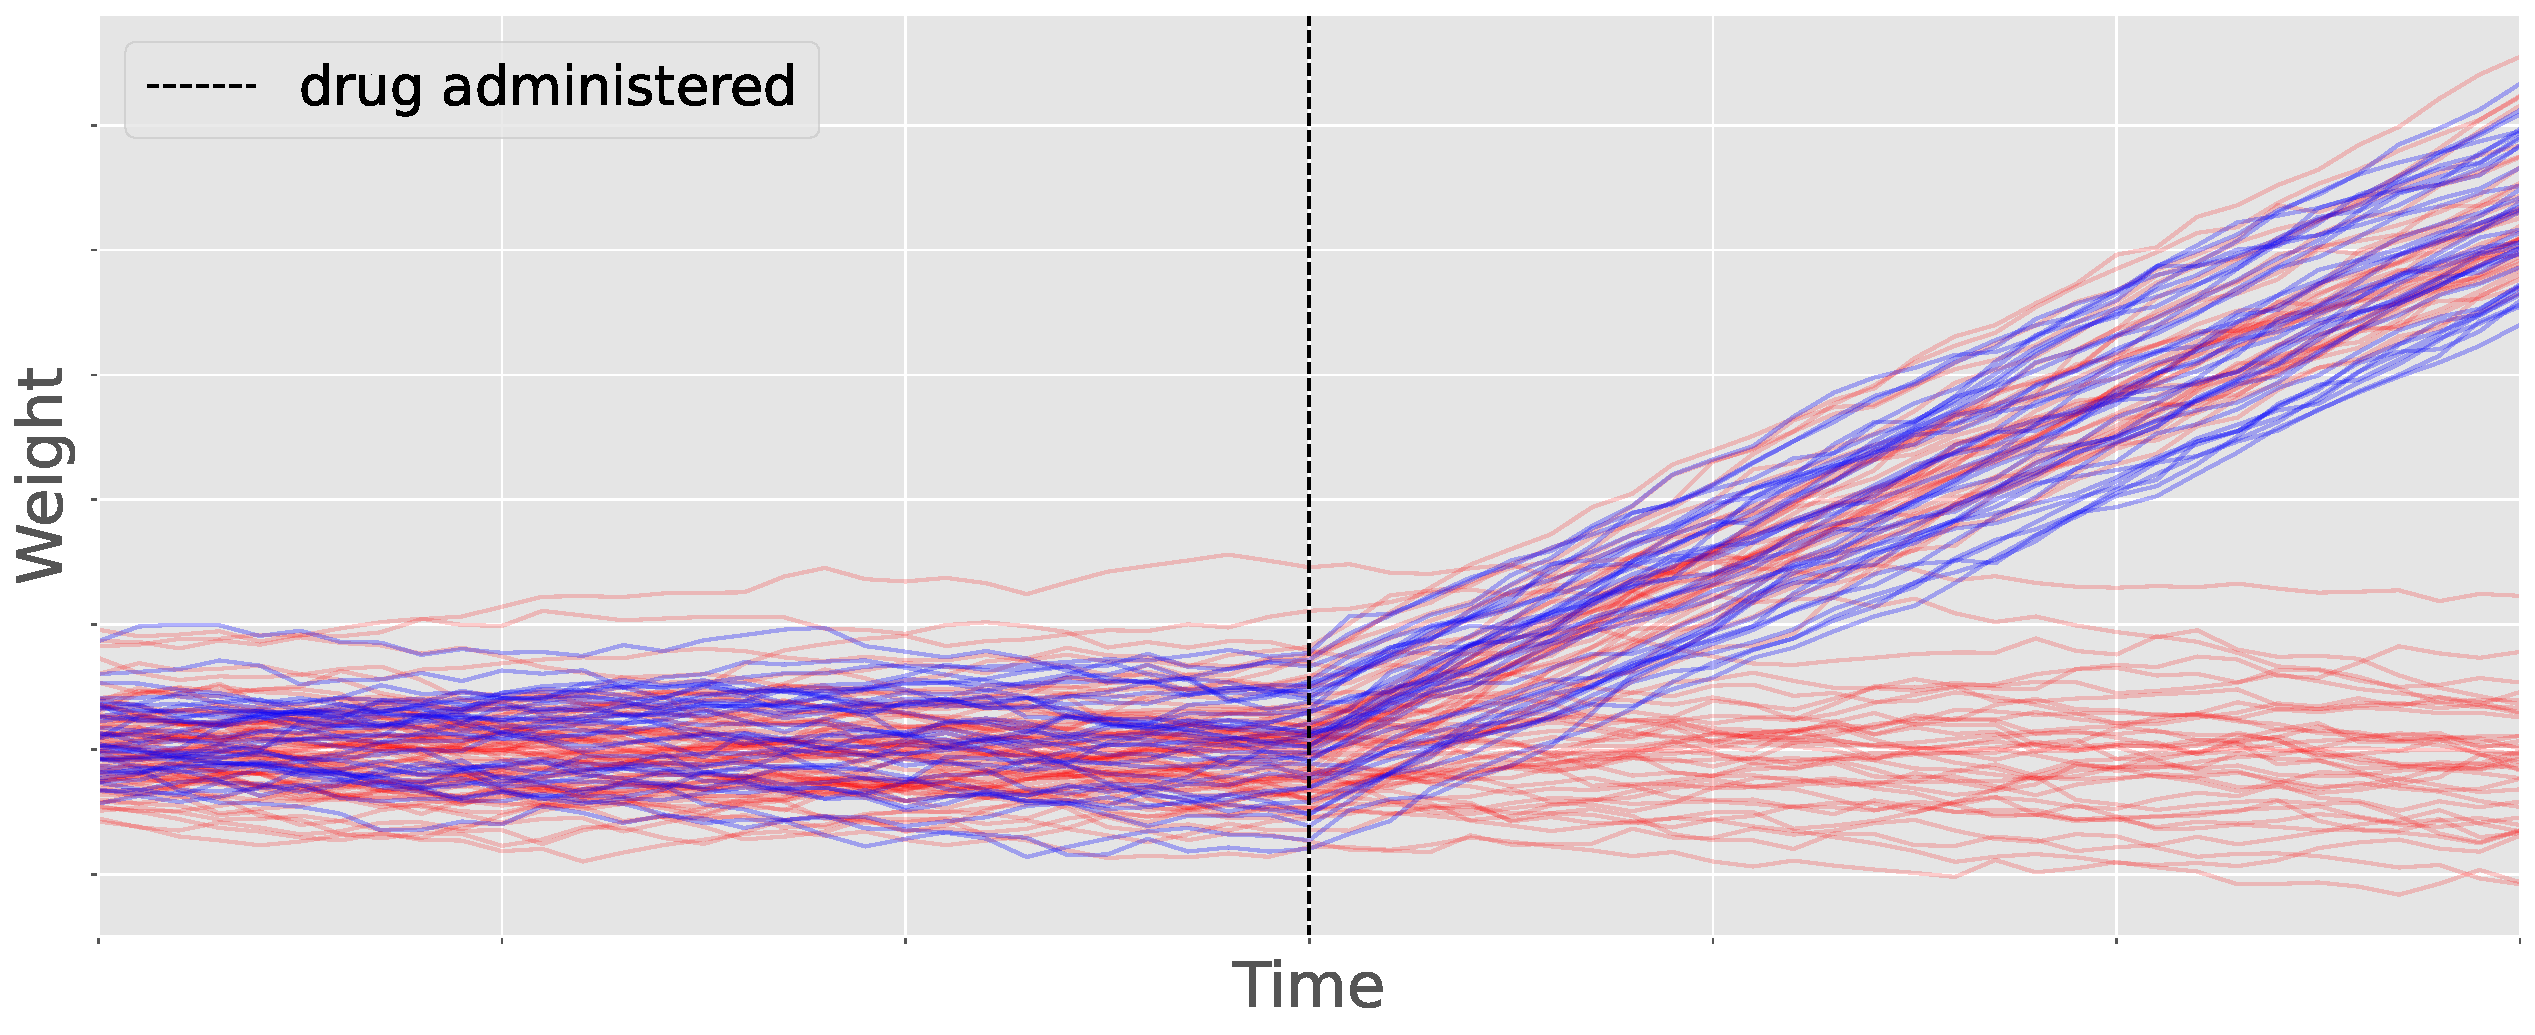
\includegraphics[height=3.3cm]{figures/causal/synthetic_example_newest2.pdf}
    \caption{The discrepancy between observational data and interventional behaviour in the presence of unmeasured confounding: the range of outcomes observed in the data for patients who were administered the drug (blue) differs from what \emph{would} be observed if the drug were administered to the general population (red).}
    \label{fig:syn_ex_intro}
\end{figure}

\begin{importantresultwithtitle}[title=Toy example: Unmeasured confounding in medical decision-making]\noindent
Suppose that we are interested in estimating the effect of a drug on the weight of patients in a certain population. 
Moreover, assume that this drug interacts with an enzyme that is only present in part of the population.
Denote by $U \in \{0, 1\}$ the presence or absence of the enzyme in a patient, and assume that when $U = 1$ the patient's weight increases after action the drug is administered, and that when $U = 0$ the drug has no effect.
Additionally, suppose that, among the patients whose data we have obtained, the drug was only prescribed to those for whom $U = 1$, perhaps on the basis of some initial lab reports available to the prescriber.
Finally, suppose that these lab results were \emph{not} included in the context $X$ captured in the observational dataset $\D$, so that the value of $U$ for each patient cannot be determined from the data we have available. 

In this setup, since the drug was only administered to patients with $U=1$, it would appear from the data that the drug causes patient weight to increase. 
However, when the drug is administered to the general population, i.e.\ regardless of the value of $U$, we would observe that the drug has no effect on patients for whom $U=0$. Figure \ref{fig:syn_ex_intro} illustrates this discrepancy under a toy model for
this scenario. In this example, since the data $\D$ contains no information about the presence or absence of the enzyme in patients, $U$, it is impossible to determine using the data $\D$ alone how the drug will affect a given population of patients. 

% Consider a medical decision-making scenario where the physician decides whether or not to administer a specific drug to the patients, and the outcome $Y$ corresponds to 
    
\end{importantresultwithtitle}


\subsubsection{Causal considerations under unmeasured confounding}
Here, we elaborate further on the implications of unmeasured confounding on the identifiability of causal effects in dynamic treatment regimes (DTRs). This topic forms the central focus of Chapter \ref{ch:5-causal} of this thesis.

\paragraph{Observational data}
Recall that in this setting, our observational data comprises trajectories obtained by observing the interaction of some behavioural agents with the real-world process.
We model each trajectory as follows.
First, we represent the action chosen by the agent at time $\tx \in \{1, \ldots, \T\}$ as an $\Aspace_\tx$-valued random variable $\A_\tx$.
We then obtain a trajectory in our dataset by recording at each step the action $\A_\tx$ chosen and the observation $\X_\tx(\A_{1:\tx})$ corresponding to this choice of action.
As a result, each observed trajectory has the following form:
\begin{equation} \label{eq:observed-data-trajectory-intro}
    \X_0, \A_1, \X_1(\A_1), \ldots, \A_\T, \X_\T(\A_{1:\T}).
\end{equation}
As outlined in the previous section, the standard off-policy evaluation methods, both in contextual bandits and DTRs, assume no unmeasured confounding in the observational dataset. Informally, this assumption holds when each action $\A_\tx$ is chosen by the behavioural agent solely on the basis of the information available at time $\tx$ that is actually recorded in the dataset, namely $\X_{0}, \A_1, \X_1(\A_1), \ldots, \A_{\tx-1}, \X_{\tx-1}(\A_{1:\tx-1})$, as well as possibly some additional randomness that is independent of the real-world process, such as the outcome of a coin toss. Unobserved confounding is present whenever this does not hold, i.e.\ whenever some unmeasured factor simultaneously influences both the agent's choice of action and the observation produced by the real-world process.


While it may be reasonable to assume that the data are unconfounded in certain contexts. For example, in certain situations it may be possible to gather data in a way that specifically guarantees there is no confounding.
Randomised controlled trials, which ensure that each $\A_\tx$ is chosen via a carefully designed randomisation procedure \cite{lavori2004dynamic,murphy2005experimental}, constitute a widespread example of this approach. However, for typical datasets, it is widely acknowledged that the assumption of no unmeasured confounding will rarely hold, and so OPE procedures based on this assumption may yield unreliable results in practice \cite{murphy2003optimal,tsiatis2019dynamic}. The following foundational result from the causal inference literature (often referred to as the \emph{fundamental problem of causal inference} \cite{holland1986statistics}) formalises this.
% shows that the value for a deterministic target policy (which always chooses a given action sequence $\ax_{1:\tx}$ regardless of the past observations $X_{0:\tx-1}(\ax_{1:\tx-1})$) is unidentifiable.
\begin{theorem}\label{thm:unidentifiability-intro}
    If $\Prob(\A_{1:\tx} \neq \ax_{1:\tx}) > 0$, then the expectation $\E[\X_{\tx}(\ax_{1:\tx})]$ is not uniquely identified by the distribution of the data in \eqref{eq:observed-data-trajectory-intro} without further assumptions.
\end{theorem}

The expectation $\E[\X_{\tx}(\ax_{1:\tx})]$ in Theorem \ref{thm:unidentifiability-intro} denotes the value at time $t$ of a deterministic target policy, which always chooses a given action sequence $\ax_{1:\tx}$ regardless of everything else.
Therefore, this result shows that the value of a deterministic target policy is unidentifiable in general, even if we have access to an infinitely large observational dataset. This also implies that the distribution of outcomes under this deterministic target policy, $\Law[X_{0:\tx}(\ax_{1:\tx})]$, is unidentifiable from the observational data distribution in general. We can also derive an analogous result for general target policies which choose actions at time $t'\in \{1, \ldots, \tx\}$ dynamically depending on past observations. 

\paragraph{Partial identification}
Since the precise identifiability of causal effects is not possible in the presence of unmeasured confounding, a notable line of work instead explores partial identification techniques \citep{manski,manski1989anatomy, manski2003partial}. Instead of the point identification of causal effects which may require strong unconfounding assumptions, partial identification typically considers the range of causal effects which may occur in the presence of confounding. For example, \cite{manski} constructs sharp bounds on the causal effects which can be readily estimated using the available observational data. While these bounds do not require any strong assumptions, they can be conservative. 

\paragraph{Sensitivity analysis}
Slightly stronger assumptions yield inferences that may be more powerful but less credible. To this end, \cite{rosenbaum2002observational} proposes a classical model of confounding for a single binary decision setting which posits that the unobserved confounders have a limited influence on the agent's actions in the real world.  \cite{namkoong2020offpolicy} extend this model to the multi-action sequential decision-making setting, and subsequently use this to obtain bounds on the off-policy value.

The Rosenbaum model is also closely related to (albeit different from) the marginal sensitivity model introduced by \cite{tan2006distributional} which also assumes bounds on the strength of unmeasured confounding on agent's actions. Subsequently, \cite{kallus2020minimax} uses the marginal sensitivity model to develop a policy learning algorithm which remains robust to unmeasured confounding. However, these confounding models impose assumptions which can be impossible to verify using observational data alone, and therefore the inferences obtained may be misleading in many cases. 

\paragraph{Proxy causal learning}
This comprises methodologies for estimating the causal effect of actions on outcomes in the presence of unobserved confounding, using \emph{proxy variables} which contain relevant side information about the unmeasured confounders \citep{xu2021deep, tchetgen2020introduction, xu2024kernel}. This usually involves a two-stage regression. First, the relationship between action and proxies is modelled and subsequently, this model is used to learn the causal effect of actions on the outcomes. \cite{kuroki2014measurement} outline the necessary conditions on proxy variables to obtain the true causal effects. While proxy causal learning may be effective in cases where such proxy variables are available, in many real-world settings the available proxy variables may not satisfy the necessary conditions for identification of true causal effects.

Chapter \ref{ch:5-causal} of this thesis considers the challenges posed by unmeasured confounding in dynamic treatment regimes. We propose a set of novel bounds on the causal effects in sequential decision-making settings, which remain valid in the presence of unmeasured confounding and rely on minimal assumptions making them highly applicable to a wide variety of real-world settings. 


% Under these confounding assumptions, we can obtain bounds on the off-policy value
% When the influence of unobserved confounding on each action is limited

% (Nonparametric Bounds on Treatment Effects)

% (PARTIAL IDENTIFICATION OF PROBABILITY DISTRIBUTIONS)

% - partial identification using proxy variables

% (Partial Identification of Causal Effects Using Proxy Variables)


% (Rosenbaum's model)

% (Nathan kallus's work)

% (emma bronstein)


% \paragraph{Proxy causal learning}

% (An Introduction to Proximal Causal Learning)

% Deep Proxy Causal Learning and its Application to
% Confounded Bandit Policy Evaluation

% - use stuff from the intro here

% Kernel Single Proxy Control for Deterministic Confounding






% \paragraph{Inferring confounders from available data}

% - Causal Effect Inference with Deep Latent-Variable Models

% - 


% - explain unmeasured confounding at an intuitive level\\
% - technical definition of unmeasured confounding\\
% - distribution of Xt and the off-policy value is unidentifiable under unmeasured confounding (also include the motivating example)\\
% - fundamental theorem of causal inference\\
% - Partial identification under unmeasured confounding\\
% - Falsification of interventional regimes using partial identification

\section{Contributions and thesis outline}
Having outlined some of the key challenges associated with Off-Policy evaluation, we dedicate the rest of this thesis to addressing each of these individually.
Specifically, this thesis is organised as follows:

\paragraph*{Chapter \ref*{ch:3-mr}: Variance reduction \citep{taufiq2023marginal}}
The first challenge we consider is that of high variance in existing OPE estimators based on importance sampling. 
As we mentioned in Section \ref{subsec:high-variance}, this variance is exacerbated in cases where there is low overlap between behaviour and target policies, or where the action or context space is high-dimensional.
To address this challenge, we propose a novel OPE estimator for contextual bandits, the Marginal Ratio (MR) estimator, which uses a marginalisation technique to focuse on the shift in the marginal distribution of outcomes $Y$
directly, instead of the policies themselves. 
Unlike the conventional approaches like IPW and DR estimators, intuitively our proposed estimator treats actions $A$ and contexts $X$ as latent variables.
As a result, the resulting estimator is significantly more robust to the overlap between policies and the sizes of action and/or context spaces.
This chapter also includes extensive theoretical and empirical analyses demonstrating the benefits of the MR estimator compared to the state-of-the-art OPE estimators for contextual bandits.
% We further illustrate the utility of the MR estimator in causal inference settings, where it exhibits enhanced performance in estimating Average Treatment Effects (ATE).

% Through rigorous theoretical analysis, we demonstrate the benefits of the MR estimator compared to conventional methods like IPW and DR in terms of variance reduction. 
% Additionally, we establish a connection between the MR estimator and the state-of-the-art Marginalized Inverse Propensity Score (MIPS) estimator, proving that MR achieves lower variance among a generalized family of MIPS estimators. We further illustrate the utility of the MR estimator in causal inference settings, where it exhibits enhanced performance in estimating Average Treatment Effects (ATE).

\paragraph*{Chapter \ref*{ch:4-copp}: Uncertainty quantification \citep{taufiq2022conformal}}
As explained in Section \ref{subsec:uncertainty-quantification}, most OPE methods have focused on the expected outcome of a policy which does not capture the variability of the outcome $Y$.
In addition, many of these methods provide only asymptotic guarantees of validity at best. 
In this chapter, we address these limitations by considering a novel application of conformal prediction to contextual bandits. 
Given data collected under a behavioral policy, we propose \emph{conformal off-policy prediction} (COPP), which can output reliable predictive intervals for the outcome under a new target policy. We provide theoretical finite-sample guarantees without making any additional assumptions beyond the standard contextual bandit setup, and empirically demonstrate the utility of COPP compared with existing methods on synthetic and real-world data.

\paragraph*{Chapter \ref*{ch:5-causal}: Causal considerations \citep{cornish2023causalfalsificationdigitaltwins}}
In this chapter we consider Dynamic Treatment Regimes (DTRs), where available observational data may suffer from unmeasured confounding. 
As mentioned in Section \ref{subsec:unmeasured-confounding}, fundamental results from causal inference mean that in this setting the interventional behaviour of outcomes, $\Law[\X_{\tx}(\ax_{1:\tx})]$, is unidentifiable from the observational distribution.  
To address this challenge, we provide a novel set of longitudinal causal bounds that remain valid under arbitrary unmeasured confounding.

Chapter \ref*{ch:5-causal} focuses on the application of these 
% We apply these 
bounds for assessing the accuracy of \emph{Digital Twin Models}.
These models are virtual systems designed to predict how a real-world process will evolve in response to interventions. 
To be considered accurate, these models must correctly capture the true interventional behaviour of outcomes, $\X_{\tx}(\ax_{1:\tx})$.
Unfortunately, the causal unidentifiability results mean observational data cannot be used to certify a twin in this sense if the data are confounded.
To circumvent this, we instead use our proposed causal bounds to find situations in which the twin \emph{is not} correct, and present a general-purpose statistical procedure for doing so.
Our approach yields reliable and actionable information about the twin under only the assumption of an i.i.d.\ dataset of observational trajectories, and remains sound even if the data are confounded.

% These bounds can be used to find the worst-case off-policy value 
% These bounds generalize the classical bounds of \cite{manski}, and can be considerably more informative in comparison.
% These bounds can be used to assess whe

\paragraph*{Chapter \ref*{ch:6-conclusion}} 
Finally, we conclude by summarising the main findings of the works presented in this thesis. 
In this chapter, we also discuss some of the limitations of our proposed methodologies and mention some interesting avenues for future research arising from these works. 

\section{An overview of work conducted during the DPhil}
In this section, we provide an overview of the research conducted during the doctoral studies by listing the papers which are included in this thesis, as well those which have been omitted.

\subsection{Works included in the thesis}
Each chapter of this thesis is based on a paper. These papers are listed in chronological order here for completeness:
\begin{enumerate}
    \item \textbf{Muhammad Faaiz Taufiq}*, Jean-Francois Ton*, Rob Cornish, Yee Whye Teh, and Arnaud Doucet.
    Conformal Off-Policy Prediction in Contextual Bandits. In \textit{\textcolor{purple}{Advances in Neural Information Processing
    Systems, 2022}}. \citep{taufiq2022conformal}
    \item Rob Cornish*, \textbf{Muhammad Faaiz Taufiq}*, Arnaud Doucet, and Chris Holmes. Causal Falsification
    of Digital Twins, 2023. Under review at \textit{Biometrika}. \citep{cornish2023causalfalsificationdigitaltwins}
    \item \textbf{Muhammad Faaiz Taufiq}, Arnaud Doucet, Rob Cornish, and Jean-Francois Ton. Marginal Density Ratio for Off-Policy Evaluation in Contextual Bandits. In 
    \textit{\textcolor{purple}{Advances in Neural Information Processing Systems, 2023}}. \citep{taufiq2023marginal}
\end{enumerate}

\subsection{Works omitted from the thesis}
For the purposes of coherence and conciseness, several works which were part of the doctoral research have been ommitted from this thesis. 
Here, we list these papers along with a brief description in chronological order for completeness. 
\begin{enumerate}
    \item \textbf{Muhammad Faaiz Taufiq}, Patrick Blöbaum, and Lenon Minorics. Manifold Restricted
    Interventional Shapley Values. In \textit{\textcolor{purple}{International Conference on Artificial Intelligence and
    Statistics, 2023}}.  \citep{taufiq2023manifold}
    \item  \textbf{Muhammad Faaiz Taufiq}, Jean-Francois Ton, and Yang Liu. Achievable Fairness on your Data
    with Utility Guarantees. Under review at \textit{NeurIPS 2024}. \citep{taufiq2024achievablefairnessdatautility}
    \item Yang Liu, Yuanshun Yao, Jean-Francois Ton, Xiaoying Zhang, Ruocheng Guo, Hao Cheng, Yegor
    Klochkov, \textbf{Muhammad Faaiz Taufiq}, and Hang Li. 
    Trustworthy LLMs: A Survey and Guideline for Evaluating Large Language Models' Alignment, 2023. 
    In \textit{\textcolor{purple}{NeurIPS 2023 Workshop on Socially Responsible Language Modelling Research (SoLaR)}}.    
    \citep{liu2024trustworthyllmssurveyguideline}
\end{enumerate}
In \cite{taufiq2023manifold}, we consider the robustness of Shapley values, which are model-agnostic methods for explaining model predictions.
Many commonly used methods of computing Shapley values, known as off-manifold methods, are sensitive to model behaviour outside the data distribution.
This makes Shapley explanations highly sensitive to off-manifold perturbation of models, resulting in misleading explanations.
To circumvent these problems, we propose \emph{ManifoldShap}, which respects the model’s domain of validity by restricting model evaluations to the data manifold.
We show, theoretically and empirically, that ManifoldShap is robust to offmanifold perturbations of the model and leads to
more accurate and intuitive explanations than existing state-of-the-art Shapley methods.

Beyond this, \cite{taufiq2024achievablefairnessdatautility} considers fairness within the context of machine learning models. 
In this setting, training models that minimize disparity across different sensitive groups often leads to diminished accuracy, a phenomenon known as the fairness-accuracy tradeoff. 
The severity of this trade-off inherently depends on dataset characteristics such as dataset
imbalances or biases and therefore, using a uniform fairness requirement across diverse datasets
remains questionable. To address this, we present a computationally efficient approach to approximate the fairness-accuracy trade-off curve tailored to individual datasets, backed by rigorous
statistical guarantees.  Crucially, we introduce a novel methodology for quantifying uncertainty in our
estimates, thereby providing practitioners with a robust framework for auditing model fairness
while avoiding false conclusions due to estimation errors.

Finally, \cite{liu2024trustworthyllmssurveyguideline} presents a comprehensive survey of key dimensions that are crucial to consider when assessing the trustworthiness of Large Language Models (LLMs). 
The survey covers seven major categories of LLM trustworthiness: reliability, safety, fairness, resistance to misuse, explainability and reasoning, adherence to social norms, and robustness. 
% Additionally, a subset of 8 sub-categories is selected for further investigation, where corresponding measurement studies are designed and conducted on several widely-used LLMs. 
The empirical results presented in this study indicate that, in general, more aligned models tend to perform better in terms of overall trustworthiness. However, the effectiveness of alignment varies across the different trustworthiness categories considered. This highlights the importance of conducting more fine-grained analyses, testing, and making continuous improvements on LLM alignment. 
% By shedding light on these key dimensions of LLM trustworthiness, this paper aims to provide valuable insights and guidance to practitioners in the field. Understanding and addressing these concerns will be crucial in achieving reliable and ethically sound deployment of LLMs in various applications.